%  article.tex (Version 1.00, released 1 October 2013)
%  LaTeX source file to demonstrate formatting for manuscripts 
%  to be submitted to SPIE journals
%  based on the class file spieman.cls, which requires 
%  the following standard packages:  times.sty, float.sty, 
%  ifthen.sty, cite.sty, color.sty, setspace.sty

%  The following commands have been added in the SPIE class 
%  file (spieman.cls) and may not be understood in other classes:
%  \affiliations{}, \sup{},\supit{}, \authorinfo{}, \keywords{},
%  \linkable and \video
%  The bibliography style file is called spiejour.bst 
%  This article.tex file needs the following image files:
%  mcr3b.eps
%  fig2.eps
%  satellite.eps

\documentclass[12pt]{spieman}  %>>> 12pt font mandatory; use this for US letter paper 
%%\documentclass[a4paper,12pt]{spieman}  %>>> use this instead for A4 paper
%%\documentclass[nocompress,12pt]{spieman}  %>>> to avoid compression of citations
%% \addtolength{\voffset}{9mm}   %>>> moves text field down
%  The following command loads a graphics package to include images 
%  in the document. It may be necessary to specify a DVI driver option,
%  for example, [dvips], but that may be inappropriate for some LaTeX installations. 
 
\usepackage[]{graphicx}
\usepackage{setspace}
\usepackage{tocloft}
\usepackage{units}
\usepackage{nicefrac}
\usepackage{color}
\usepackage{epstopdf}
\usepackage[globalcitecopy,labelstoglobalaux,sectionbib]{bibunits}
\usepackage[thinspace,thinqspace,squaren]{SIunits}
\usepackage{fancyhdr}
\usepackage{url}
\usepackage{wasysym}
%\usepackage{alltt}
%\renewcommand{\ttdefault}{txtt} 
\usepackage{array}
%\usepackage[version=3]{mhchem}
%\usepackage[T1]{fontenc}
%\usepackage{textcomp}
%\usepackage{verbatim} 
%\usepackage{mathpazo}
%\usepackage{amsmath} %>>> for AMS math formatting including bold Greek symbols
%\usepackage{mathtools}
\usepackage{amssymb}
\usepackage{accents}
%\usepackage{hyperref}
\usepackage{url}
\usepackage{amscd}
\usepackage{epsfig}
\usepackage{cite}
\usepackage{subfig}
\usepackage[globalcitecopy,labelstoglobalaux,sectionbib]{bibunits}
%\usepackage[sectionbib]{bibunits}
\usepackage{appendix}
\usepackage{slashbox}
\usepackage{multirow}
\usepackage{pbox}
%\usepackage{caption}
\usepackage{pdflscape}
\usepackage{nicefrac}
\usepackage{rotating}
\usepackage[colorlinks=true,citecolor=blue,urlcolor=blue,linkcolor=blue,
		pagebackref,
		hyperindex,%linktocpage,
		bookmarksnumbered=true,bookmarksopen=true,bookmarksopenlevel=0,
		pdfstartview=FitV,
		pdfstartpage=1]
	{hyperref} % makes pdf look nice with hyperlinks

\title{Working title: the most amaz-zing SPIM and how we built it.} 

\author{M. Caroline M\"{u}llenbroich,\supscr{a,b} Ludovico Silvestri, \supscr{a,c} Leonardo Onofri,\supscr{e} Irene Costantini,\supscr{a} Marcel Van t'Hoff\supscr{f} Leonardo Sacconi,\supscr{a,c} Giulio Iannello,\supscr{e} Francesco S. Pavone,\supscr{a,b,c,d}  }

\affiliation{\supscrsm{a}European Laboratory for Non-linear Spectroscopy (LENS), University of Florence, Italy\\
\supscrsm{b}Department of Physics and Astronomy, University of Florence, Italy\\
\supscrsm{c}National Institute of Optics, National Research Council, Italy\\
\supscrsm{d}International Center for Computational Neurophotonics (ICON Foundation), Italy\\
\supscrsm{e}Integrated Research Centre, University Campus Bio-Medico of Rome, Italy\\
\supscrsm{f}Distrio, Murmex}

%%%%%%%%%%%%%%%%%%%%%%%%%%%%%%%%%%%%%%%%%%%%%%%%%%%%%%%%%%%%% 
\renewcommand{\cftdotsep}{\cftnodots}
\cftpagenumbersoff{figure}
\cftpagenumbersoff{table} 
\begin{document} 
\maketitle 

%%%%%%%%%%%%%%%%%%%%%%%%%%%%%%%%%%%%%%%%%%%%%%%%%%%%%%%%%%%%% 
\begin{abstract}
200 words limit. no numerical references presenting concisely the objectives, methodology used, results obtained, and their significance.
\end{abstract}

%>>>> Include a list of up to six keywords after the abstract
\keywords{Light sheet microscopy, Big data, Optical clearing, Data management, whole brain imaging, rolling shutter, 7,8.}

%>>>> Include contact information for corresponding author
{\noindent \footnotesize{\bf Address all correspondence to}: First author, University Name, Faculty Group, Department, Street Address, City, Country, Postal Code; Tel: +1 555-555-5555; Fax: +1 555-555-5556; E-mail:  \linkable{myemail@university.edu} }
%%%%%%%%%%%%%%%%%%%%%%%%%%%%%%%%%%%%%%%%%%%%%%%%%%%%%%%%%%%%%

%\begin{spacing}{2}   % use double spacing for rest of manuscript

%%%%%%%%%%%%%%%%%%%%%%%%%%%%%%%%%%%%%%%%%%%%%%%%%%%%%%%%%%%%%
\section{Introduction}%funnel shape
\label{sect:intro}  % \label{} allows reference to this section

The highly ambitious project of mapping and understanding each and every neuronal connection in the whole brain has been moved from the realm of wishful longing to feasible reality by the recent advent of light sheet fluorescent microscopy (LSFM). With this technique 3D data sets can be acquired with a resolution that is high enough to identify neurons and their dendritic, axonal and spine features in time scales which are no longer the bottle neck of high-throughput acquisition. In LSFM, the sample is illuminated with a thin sheet of light confined into the focal plane of the detection objective, which collects the fluorescence emission along an axis perpendicular to the illumination plane\cite{Huisken2009}. This technique drastically reduces the imaging acquisition time by recording millions of pixels in parallel and affords optical sectioning by operating fluorescence excitation and detection on separate, perpendicularly oriented paths where the excitation light sheet and the detection focal plane overlap (Figure\ref{fig:Panel1},A). Consequently fluorophores outside the light sheet are neither bleached nor contribute blurring out-of-focus noise. Consequently LSFM reduces phototoxicity and photobleaching while achieving excellent resolution at high penetration depths; however, it requires the sample to be transparent. 

Several challenges remain to be overcome, however, to allow fast and, most of all systematic, production of reliable datasets and their meaningful interpretation to further our understanding of neuronal networks. Those challenges include fast, cheap and reproducible sample preparation, automated image acquisition that does not require constant attention by an expert and, most crucially, the storage, interpretation and analysis of the unprecedented huge data sets light sheet microscopy routinely produces. The mapping and understanding of this ``big data" is a colossal task that requires the expertise of computer scientists to employ fully automated post-processing, for example, to do cell counting or blood vessel segmentation. On the other hand, the imaging of large, intrinsically opaque samples in light sheet microscopy necessitates clearing protocols based on refractive index matching which render the tissue transparent. This makes LSFM a truly interdisciplinary field in which the technological advances by optical developers need to be matched by novel development in the area of information and biotechnology.

Here we will review a state-of-the-art LSFM, as it is implemented in our lab, which can be used to acquire 3D data sets of clarified mouse brains. The LSFM features double-sided illumination with a digitally scanned light sheet and a sample chamber which has been specifically designed for the the imaging of large ($> 1cm^3$), immersed and freely movable samples. After briefly presenting the optical clearing protocol we employ to render our samples transparent, we explain how to prepare and mount the samples for stable, 3D imaging for several days. In addition to a detailed description of all opto-mechanical components, we further present a practical guide for the alignment of a LSFM, a non-trivial task which in previous publication has too often been summarised in a single sentence. A systematic approach to handle, store and analyse the data is also given. We further explain about the data volume we produce how it can be reduced and handled. We finish with some nice data and an outlook.  The final sentence of the introduction needs to be amazing. 


\begin{figure}
   \begin{center}
   \begin{tabular}{c}
   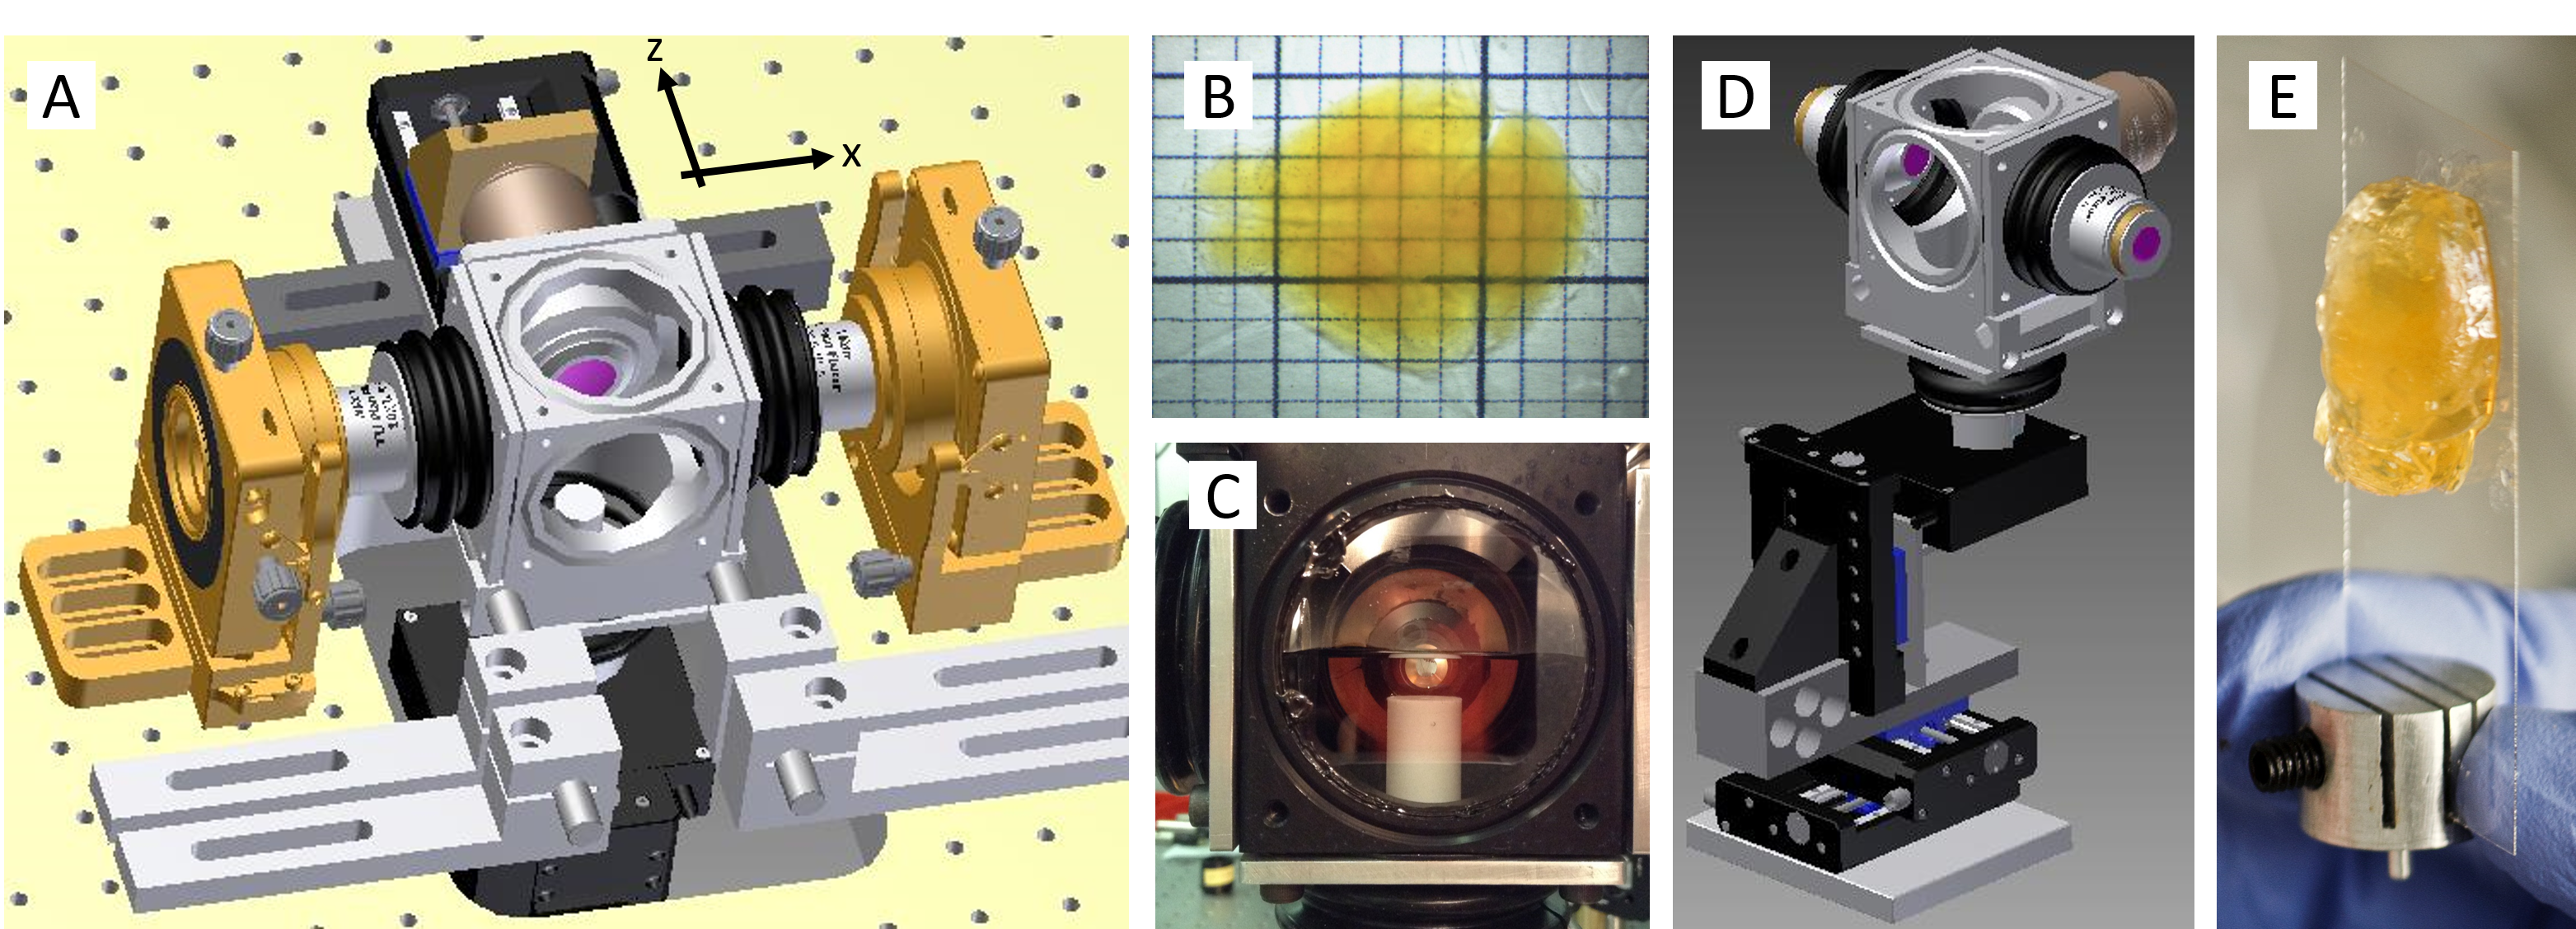
\includegraphics[width=\textwidth]{Panel1.eps}
   \end{tabular}
   \end{center}
   \caption{\label{fig:Panel1} Schematic of light sheet microscopy. (A) Fluorescence excitation (along x axis) and detection (along z axis) are operated on independent, perpendicular light paths where the excitation light sheet and the detection focal plane overlap. The clarified, fluorescently-labelled brain (B) is mounted on a Teflon cylinder inside the watertight chamber (D) and can be translated and rotated freely with piezo motors (D). The sample is glued onto a cover slip which is slid into a custom made adapter mount that is inserted into the Teflon cylinder (E).} 
   \end{figure}

\section{Optical clearing and sample mounting}
Biological tissue is, bar of very few exemptions like the cornea or zebrafish larvae, highly scattering. Scattering is the deflection of light rays due to the heterogeneous mixture of cells and sub-cellular structures with varying refractive indices. Rayleigh scattering, the nearly isotropic and strongly wavelength dependent scattering of light by particles much smaller than the wavelength of light, and Mie scattering, which occurs on cellular structures such as organelles and other refractive structures which are larger than the wavelength of light, far outweigh absorption and cause most biological tissues to be opaque. In the visible spectrum, the scattering of fluorescence photons is dominant over ballistic fluorescence such that for the imaging of large samples optical clearing methods based on refractive index matching have been employed. These methods involve several chemical sample preparation steps to generate transparent yet structurally and anatomically intact tissue.

A successful optical clearing method not only renders the tissue transparent but also causes neither quenching of protein fluorescence nor tissue distortion and is compatible with repetitive immunostaining. A very promising method called CLARITY\cite{Chung2013,Tomer2014} transforms tissue into a nanoporous, hydrogel-hybridized, lipid-free form. Crucially for high through-put clearing and imaging of large samples, the protocol, however, is ideally also fast, easy and cheap. Our lab therefore development a versatile, simple, rapid and inexpensive clearing method based on a water-soluble agent, 2,2'-thiodiethanol (TDE) which in combination with CLARITY allows for the optical clearing of entire mouse brains or human biopsies. With this protocol (see [cite Irene] for a detailed description) a mouse brain (Figure\ref{fig:Panel1},B) takes 1 month to clear at a costs of \$XY.
		
To elucidate neuronal projections and functional connections in structurally intact tissue it is paramount to be able to image centimeter-sized, clarified samples, such as mouse brains, with high resolution in whole mount preparation. The question of sample preparation and mounting in light sheet microscopy is not trivial but requires novel approaches to such extent that it is becoming a separate field of research and very diverse strategies such as FEP tubes, 3D printed chambers and Quarz cuvettes have been reported (cite), however these approaches are limited to much smaller sample volumes. 
	
We designed a cubic, water-tight sample chamber (Figure\ref{fig:Panel1},C) that allows access from all six sides while maintaining the 3D integrity of large, clarified and fluorescently-labelled mouse brains. A motorized x-, y-, z-, $\theta$-stage (M-122.2DD and M-116.DG, Physik Instrumente) allows free 3D motion and rotation of a Teflon cylinder which reaches into the centre of the chamber (Figure\ref{fig:Panel1},D). The clarified brains are fixed with super glue to a coverslip which is slid into a custom made adapter and tightened with a plastic-capped screw. The adaptor is then inserted into the Teflon cylinder (Figure\ref{fig:Panel1},E) with the coverslip being positioned on the far side of the detection objective. Three different slits in the adapter correspond to varying distances to the detection objective and give variability in sample thickness for example to allow also for the mounting of rat brain hemispheres. The clarified brains are imaged immersed in clearing solution composed of 63\% TDE in Phosphate buffered saline (PBS) and a refractive index of 1.45. Stable mounting is a key concern as a whole brain tomography can require image acquisition in excess of 3 days. We found that the effect of gravity, tissue shrinking/expansion and evaporation of PBS over such time spans are negligible, however, after that point the super glue is starting to dissolve.		
		
	\section{Optical path}

	\subsection{Illumination}
		
		\begin{figure}
   \begin{center}
   \begin{tabular}{c}
   \includegraphics[width=\textwidth]{Panel2.eps}
   \end{tabular}
   \end{center}
   \caption{\label{fig:excitation} (A) Topview of the excitation path. The galvo scanners are mounted above periscopes. LP: long-pass filter, I: iris, AOTF: acousto-optical tunable filter, LM: laser modulator, PBS: polarisation beam splitter, ABCD: flip mirrors. Inset: detection. (B) Oblique view of the microscope. A custom-made breadboard serves to mount the sample chamber and objectives at an elevated height and features two circular holes at the edges for the periscopes and a large central cut out for the translation stages. A second breadboard is used for the camera.} 
   \end{figure}
		
The custom-made, confocal light sheet microscope is equipped with 5 linearly polarised, cw lasers for fluorescence excitation (Figure\ref{fig:excitation},A). The wavelengths were chosen to excite the most common fluorophores (see Table\ref{tab:optomechanics} for the manufacturer and specifications of opto-mechanical components) and have each an output power of 50mW. The laser light from each laser is first collimated and expanded with a telescope (f140, f200) and then combined into a common path with a beam steering mirror and a long-pass filter (Semrock, LaserMUX\texttrademark\ series). An acousto-optical tunable filter (AOTF) acts as fast ($\mu s$) electronically tunable filter which uses the acousto-optical interaction inside an anisotropic medium to select and transmit any combination of up to four of the laser lines. The radio-frequency applied on the AOTF transducer controls the wavelength being transmitted into the first order and the radio-frequency amplitude allows to adjust the transmitted light intensity. Due to the nonlinear response of the AOTF we measured the AOTF light transmittance for each wavelength as a function of radio frequency amplitude and determined a linear look-up table through interpolation. The zero order light is blocked by an iris. An electro-optical laser modulator acts like a wave plate with electrically controlled retardation and rapidly rotates (hundreds ns/ms?) the input polarisation of the excitation light by $90\degree$. The wavelength-dependent, high voltage that needs to be applied to the birefringent crystal inside the modulator to change the optical path length is provided by a two-step pre-amplification system. First, a low voltage, analog signal from the DAQ board is pre-amplified with custom made electronics and then fed into a commercial high voltage amplifier. A digital line is used to electronically control the frequency of the polarisation shift. After the laser modulator the excitation beam is further expanded by a factor of 2 (f100, f200) with two achromatic doublets. From here on three different light paths can be chosen through flip mirrors. One light path option guides the light through an axicon (apex angle of $160\degree$) and an achromatic doublet (f50) to create a Bessel beam. The other two options create Gaussian beams of different beam diameter. This diameter variation translates to different fields of view later on in the detection path. The three options are recombined before a polarising beam splitter cube which splits the excitation light depending on its polarisation into one of the two excitation arms which are built to be identical. The beam is reduced with a telescope (f350, f200) whose telecentric plane coincides with the mirrored surface of a galvanometric scanner (galvo). The galvos are mounted on a custom made optical breadboard which features two circular holes to pass the periscopic beams and a large central cut-out for the sample chamber and motor stages. The light sheet is generated digitally by scanning the excitation beam with a sawtooth signal applied to the galvo. This generates perfectly incoherent illumination resulting in fewer artefacts.%cite{StelzerNatMeth2014}.
The scan mirror surface is reimaged with a telescope (f50, f100) onto the back aperture a long working distance, low magnification objective (Nikon, 10x 0.3NA WD 17.5mm). The two excitation objectives are designed for air immersion. A coverslip glued to the front housing edge serves the dual purpose of maintaining the first diffractive surface between the front optical element and the air and to protect the glue/mounting of the lens elements which is compromised by the organic solvent. The sample chamber is tightly bolted  to the optical breadboard while soft connections through silicone bellows allow for adjustive movements of the objectives and free 3D motion of the motor stages. All connections are sealed with rubber rings and silicone caulk and additionally tightened with cable binders. In this way the objectives can be refocused and realigned without compromising the watertight seal of the chamber. 

	
		\subsection{Detection}
		%objective, camera, rolling shutter. Use references\cite{Silvestri2012} to old SPIM.
		
		Fluorescence is collected on a axis perpendicular to the excitation with an objective that was specifically designed for immersion in clearing solutions of various refractive indices. The objective is equipped with a correction collar allowing for immersion in media with refractive indices ranging from 1.41 to 1.52 (Olympus, XLSLPLN25XGMP). To image the whole volume of interest the objective has a relatively low magnification of 25x and a large working distance of 8mm yet a high numerical aperture (1.0NA) affords high resolution imaging. HERE WE'LL NEED SOME CHARACTERISATION DATA. An overview of imaging properties and derived quantities is given in Table\ref{tab:resolution}. We use a tube lens of 200mm to create an image on a sCMOS camera (Orca Flash4.0, Hamamatsu). A fluorescent filter is used to block out any excitation light. The camera chip of over 4 megapixels is read out in one sweep from top to bottom in the so-called light sheet mode in which only a subset of horizontal lines is exposed and consequently read out and any time. This sweeping line exposure creates a virtual confocal slit. Confocality is achieved by synchronising a single line which generates the light sheet with the exposure of a few lines on the CMOS chip.
		
For image acquisition the sample is slowly translated at a fixed speed along the detection axis through the light sheet. Images are recorded at a frame rate of 44Hz in different planes along the optical axis of the detection lens (here z) to acquire a stack. After successful stack acquisition the sample is moved to an adjacent vertical position (here y) to acquire the next image stack. Once the entire vertical slice composed of z stacks is acquired the sample is moved to an incremented x position. In this way the entire cubic volume is imaged. 
	
	\subsection{Alignment}

\begin{figure}
   \begin{center}
   \begin{tabular}{c}
   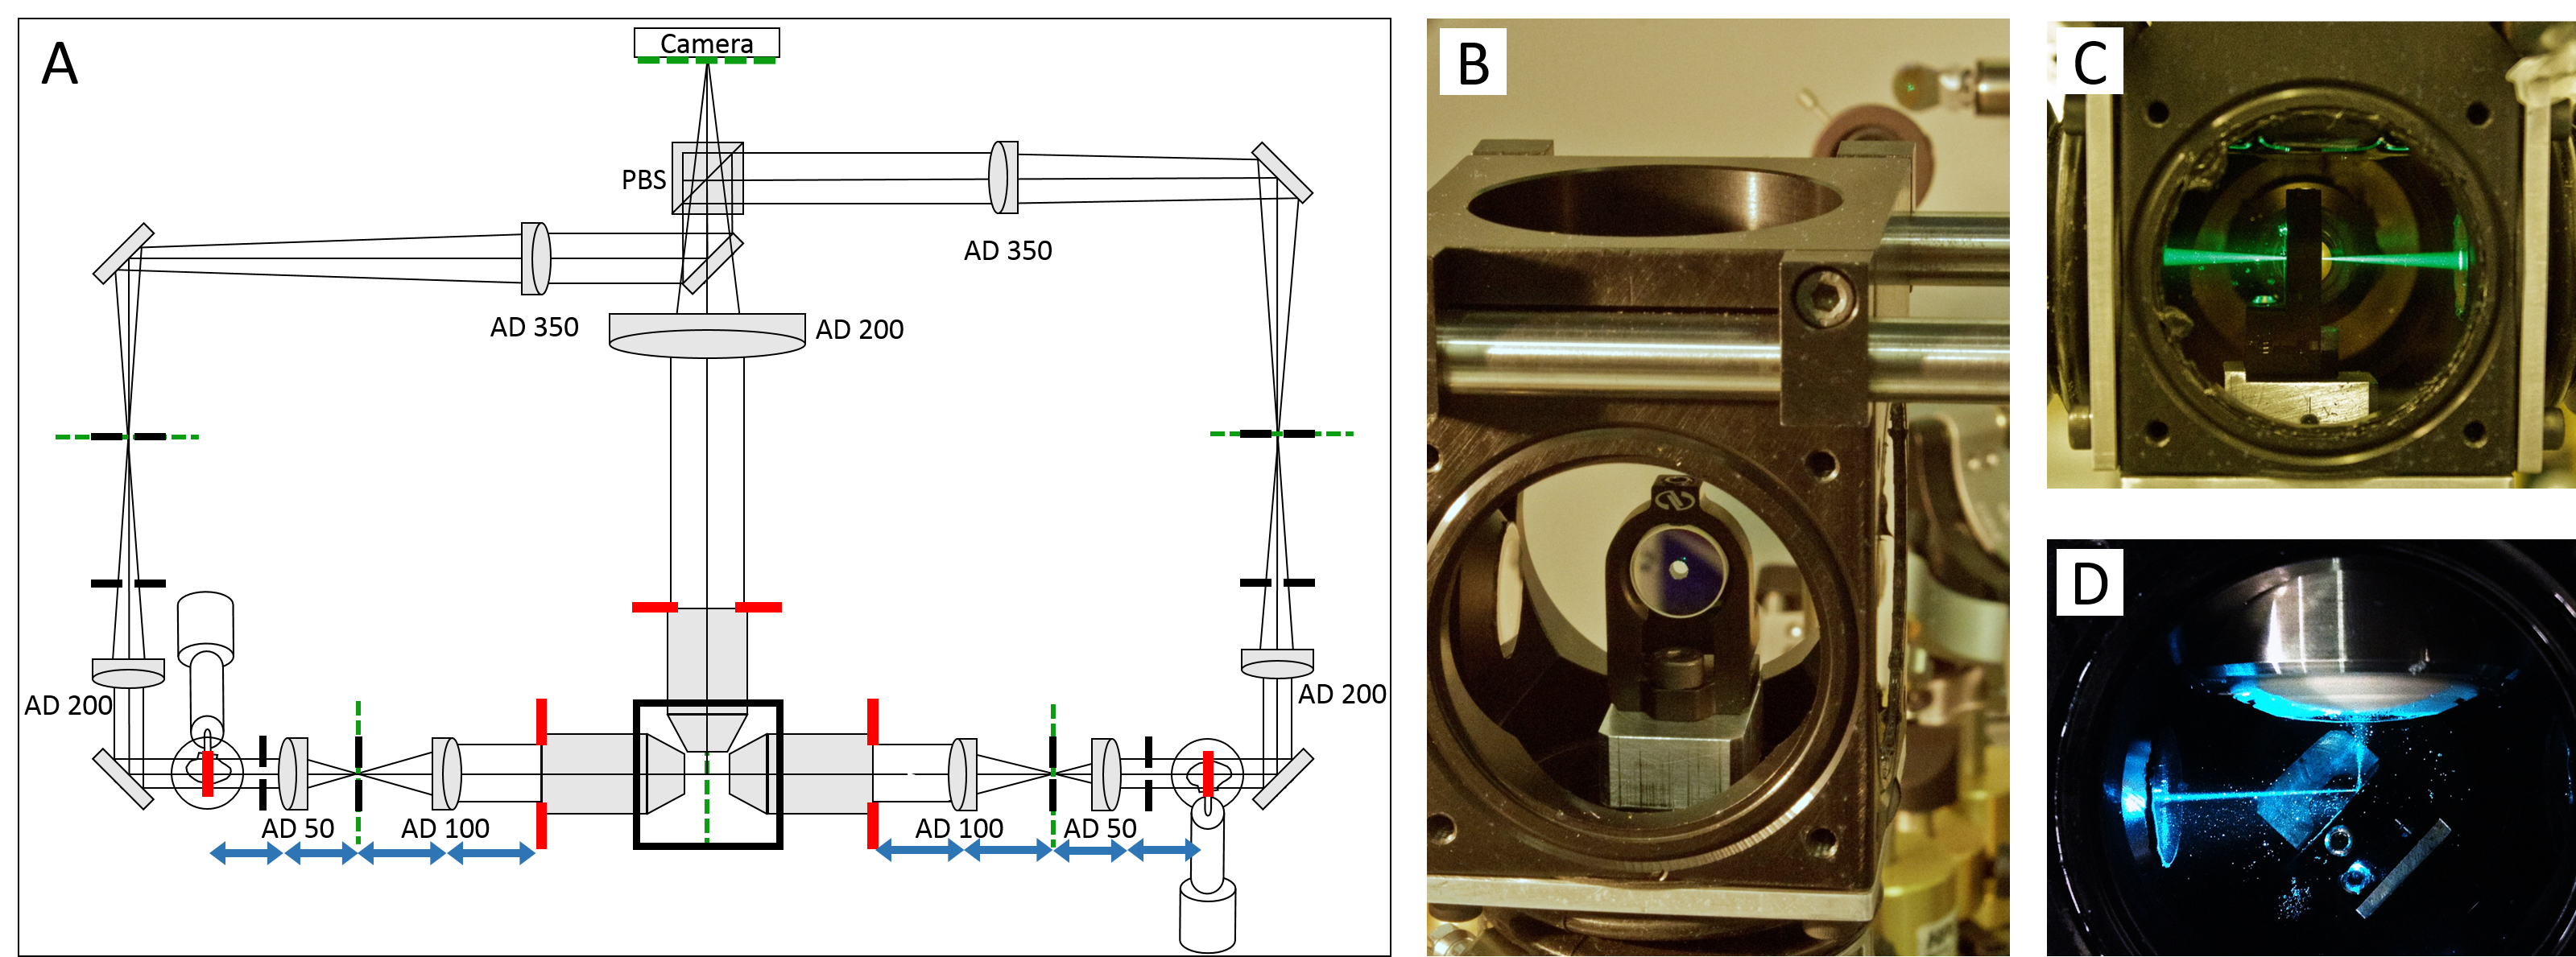
\includegraphics[width=\textwidth]{Panel3.eps}
   \end{tabular}
   \end{center}
   \caption{\label{fig:alignment} (A) Basic geometrical optics of a double-sided illumination light sheet microscope. AD: achromatic doublet, PBS: polarising beam splitter, red: objective back focal planes and conjugated telecentric planes, green: image planes, blue: 4f telecentric lens system. (B) The alignment mirror can be rotated to precisely reflect at $45\degree$. (C) With lateral movement the alignment mirror can be placed such that light is transmitted into the opposing excitation arm. (D) Alignment mirror with drilled hole for light transmission, mount for tip adjustment and adaptor for the Teflon tube.} 
   \end{figure}

For light sheet microscopy it is crucial that excitation and detection occur on perpendicular axes because any deviation from this geometry results in obscured images of reduced resolution and contrast. The objectives need to be perfectly confocal so that the fluorescence that is generated in the swept excitation beam also falls within the detection objective's depth of field. Telecentricity, that is the imaging with two lenses which are the sum of their focal lengths apart, has to be strictly observed in all three arms (Figure\ref{fig:alignment},A), which means the galvo scanners need to be precisely placed in telecentric planes of the excitation objectives while in the detection path, the camera chip needs to be positioned in an image plane of the detection objective. Additionally, homogeneous illumination from both sides impose strict symmetry considerations on both illumination arms that have not only to be sufficiently aligned within themselves respectively but function as pair with recursive dependence. 

Our microscope was aligned with two tools, a shear plate to qualitatively assess collimation and a small mirror that can be mounted inside the sample chamber where the sample would usually be. The 0.5in mirror was first pierced with a drill using a ceramic drill bit to produce a hole roughly in its centre of the approximately the same diameter as the excitation beam inside the sample chamber. Using a compact single axis adjustable mirror mount (V50-AX, Newport) attached to the Teflon cylinder inside the chamber allows to to adjust the pitch of the reflection with the mount and the yaw with the rotation stage while at the same time providing a very space efficient mounting for the pierced 0.5in mirror. With this ``sample mirror" three different position can now be easily implemented, firstly, back reflection by hitting the reflective surface at $0\degree$, secondly, transmission by laterally displacing the mirror until the light passes through the drilled hole, and thirdly, reflection of the light by $90\degree$ by precisely turning the mirror mount by $45\degree$ using the rotation stage. 

\begin{figure}
   \begin{center}
   \begin{tabular}{c}
   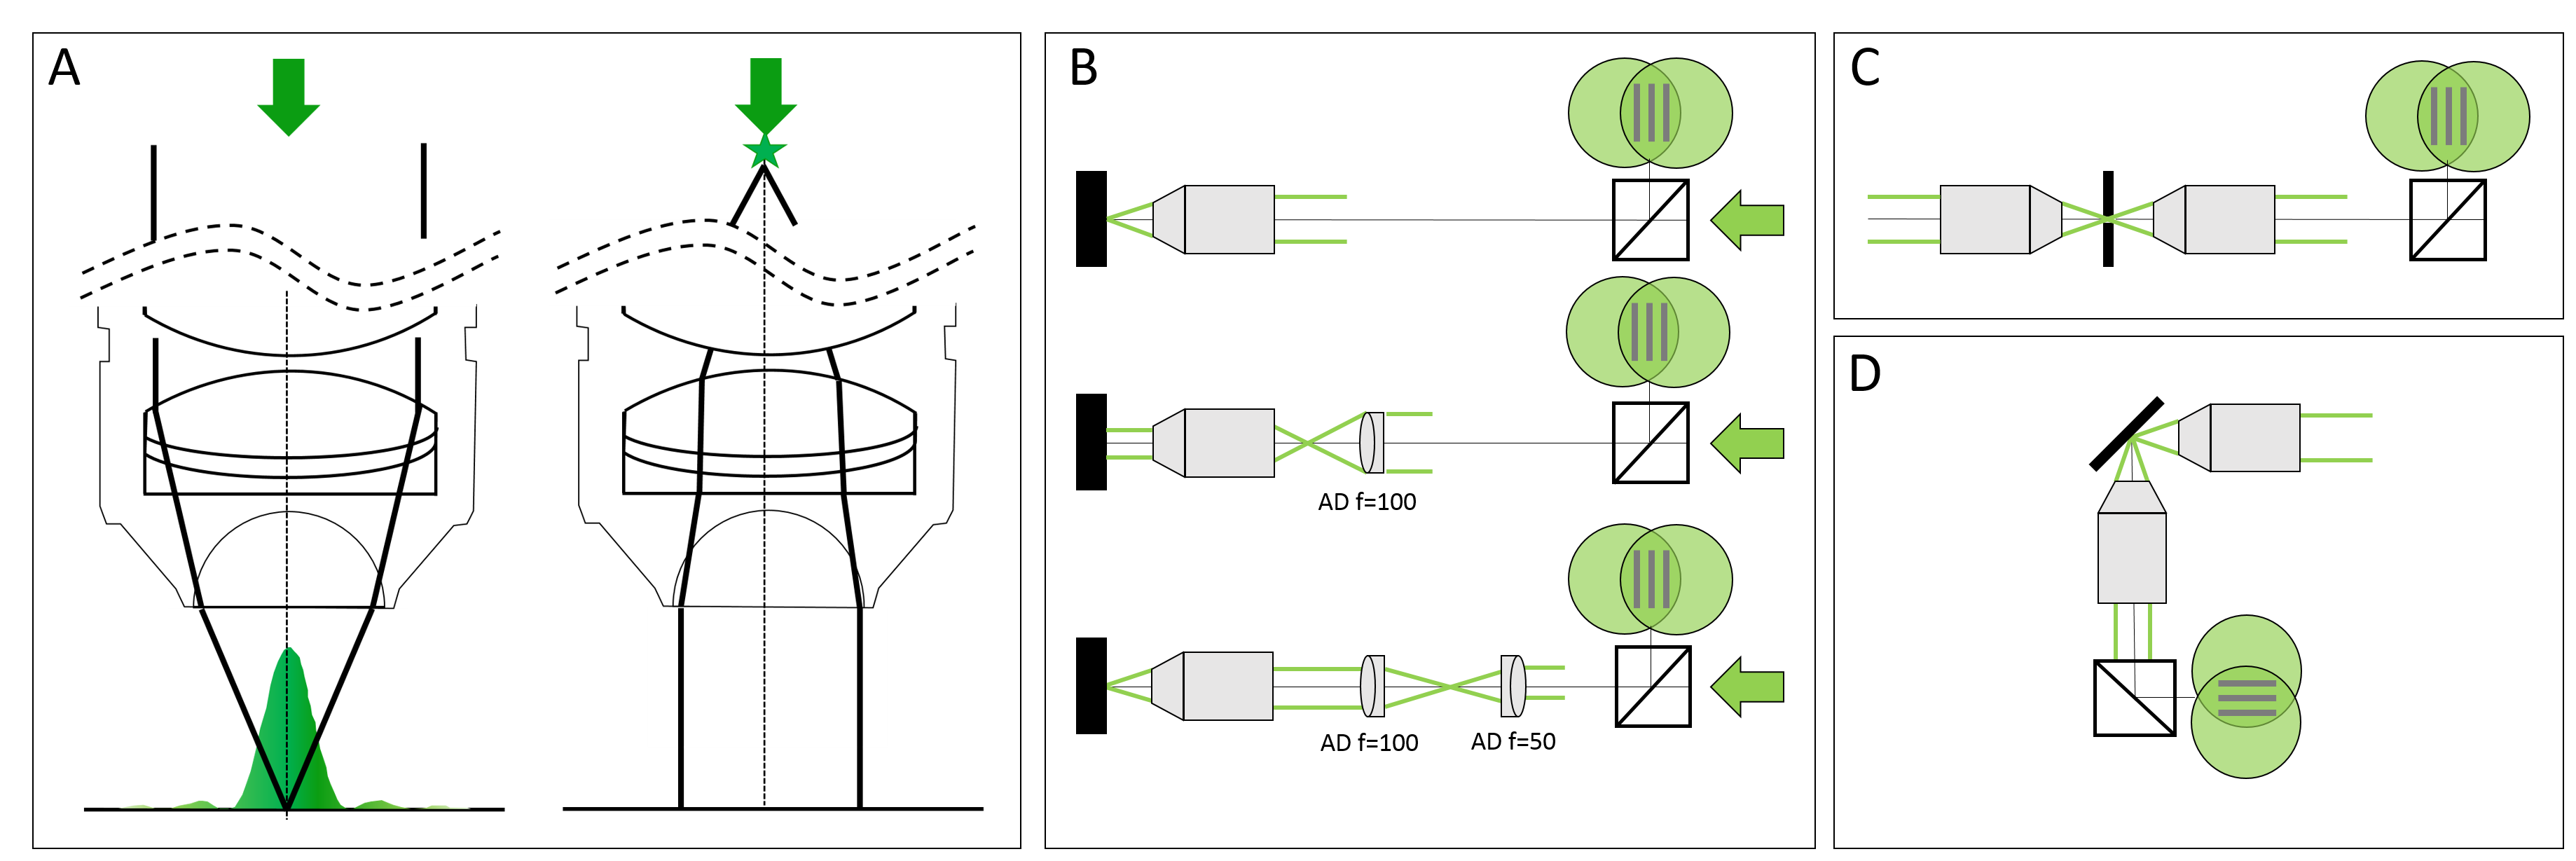
\includegraphics[width=\textwidth]{Panel4.eps}
   \end{tabular}
   \end{center}
   \caption{\label{fig:alignment2} (A) Working principle of a microscope objective (left): a collimated input beam in converted into a spherical wavefront. Right: inverted light path where a focal spot in the back aperture creates a collimated output. (B) Recursive placement of lenses using the sample mirror in back-reflection mode, (C) in transmission mode and (D) in reflection mode.} 
   \end{figure}

The excitation objectives are fixed on mounts which allow three dimensional translation plus pitch and yaw adjustment (LP-1A, Newport). In a first step the beam paths of both excitation arms where brought to overlap through irises placed on the breadboard and the optical bench without any microscope objectives. We found it useful to use two mirrors in each periscope, one vertically mounted and one mounted at $45\degree$ for vertical deflection of the incoming beam. In this way full beam steering can be achieved to realign the periscope before hitting the galvo scanner. After this initial alignment the first excitation objective was then placed into the beam path and brought to focus onto the sample mirror, which was adjusted to reflect the light back into the same objective. Using a shear plate and a polarising beam splitter cube the back reflected light was qualitatively checked for collimation to ensure the sample mirror was correctly placed in the focal plane of the objective (Figure\ref{fig:alignment2},B). The sample mirror was then moved laterally to allow the excitation beam to pass through the drilled hole and the second excitation objective was placed (Figure\ref{fig:alignment2},C). This time collimation was checked with the light going through both objectives and so their confocal placement was insured. The microscope was then aligned recursively by starting at the confocal point between the objectives and placing successively lens after lens in the up-stream direction. Finally, the sample mirror was position in reflection mode and the detection objective was aligned (Figure\ref{fig:alignment2},D). 

	
\section{Software Management}

	\begin{figure}
   \begin{center}
   \begin{tabular}{c}
   \includegraphics[width=\textwidth]{connectivity.eps}
   \end{tabular}
   \end{center}
   \caption{\label{fig:connectivity} Connectivity scheme} 
   \end{figure}

%Here we describe all things software control and communication, components and their interaction. how is the rolling shutter timed with galvos, triggers and clocks etc.


%Based on a modular scheme (OOP) using Murmex development kit
%Separate building blocks control different components of the microscope
%Hierarchical structure coordinates complex tasks
%Communication takes place through RabbitMQ server (open source message-oriented middleware) using the LabbitMQ library

The microscope was designed and developed by optical technology specialists yet needs to be operational in a multi-user environment. The greatest challenge consists in making the use of the microscope easy and intuitive such that no formidable expertise is needed when it is operated by interdisciplinary researchers. Another aspect of software design is avoiding redundancy in writing software, for example, when a second or third microscope with basic similarity yet slightly specialised equipment is being designed in the same laboratory. Writing well structured scientific software in a group of researchers is an often recurring challenge. The final code should be the common effort of all contributors each with their own know-how and practical expertise. Contemporary experimental research often relies on the acquisition and real-time processing of various data streams. In a given experiment, data may be acquired from multiple, even spatially separated sources, while individual processing steps may be computationally intensive and need to be distributed over several computers to be performed on-line. We chose to write our software in LabVIEW (National Instruments), as this language is particularly well suited to hardware control and data acquisition by pre-developed methods, using the Murmex library. The Murmex library, developed by one of the co-authors, helps users to collaborate on software development by letting them independently create their respective contributions to the software within a standardized programming scheme by employing object oriented programming methodology (OOP). Murmex uses the library LabbitMQ, which is a wrapper of RabbitMQ, a message-oriented middle ware facilitating message shipment and receival. These layers of abstraction are mostly hidden for the developers.

\subsection{Object oriented programming}
In OOP the developer creates classes, which are data structures that contain private data and methods that perform actions on the data. LabVIEW supports classes since 2006, but got to its mature form with LabVIEW 2009. When you create a subclass (child) from the toplevel class (parent), you automatically inherit its methods and data. Public methods can be called by the child, while private methods are only accessible by the owning class. A method implemented by the parent, which has the Dynamic Dispatch enabled and is public, can be replaced or augmented by the child. The parent can force the child to call its method or allow to ignore its code. A call to such a dynamic and public method is chained, it thus calls first the child method, which perform the action before or after calling the parent. The parent calls again its parent before or after executing its code and thus create a complete call chain for a single method.
Next to the methods, the classes have private class data, which can only be accessed by the owning class. In order to give access to its data, a method needs to have methods accessing the data. The instance created at runtime from a class is called the object. Many objects can be made from a class, like many pies can be made from a pie recipe. Next, each object runs independently and contains its own data.


\subsection{RabbitMQ}
The RabbitMQ server (message broker) needs to be installed either locally or somewhere in the network. The message-based communication allows for buffered, asynchronous and reliable message communication between several software components. Messages are routed by the broker to the specific software component by its ID. In order to access the functionality of RabbitMQ, the application programming interface (API) \href{http://sine.ni.com/nips/cds/view/p/lang/en/nid/211065}{LabbitMQ} was used, which uses .NET calls for sending and receiving messages to and from the RabbitMQ broker. Messages can be sent to a single recipient by its ID or sent to all available components.

\subsection{Murmex}
The \href{http://sine.ni.com/nips/cds/view/p/lang/en/nid/212895}{Murmex library} is a software development kit for creating distributed finite state machines in LabVIEW (2012 and newer). A finite state machine resembles the Strategy pattern [Design Patterns: Elements of Reusable Object-Oriented Software, E. Gamma, R. Helm, R. Johnson, J. Vlissides, 1994], which lets the software of one component proceed from one particular state to another based on message it receives from itself or other components (for example to execute Initialise, Start, Proceed, Stop, Terminate). In each state it executes the code for that state only, but flexible execution patterns are possible. It thus allows for predictable behaviour, without knowing the exact code. Murmex has twelve pre-defined common states (e.g. Initialise, Start, Stop, Terminate) and a generic state for implementing custom states. A software component that represents one, yet large, task, often uses only those previously four mentioned states. Examples for such a software component are the implementation of a laser, a translation stage and a camera. Such a component would implement in the Initialise method the initialisation of the communication port to the device, start activity in the Start method, stop activity in the Stop method and close the communication and free up memory in the Terminate. 
While each component is an autonomous program, variables on which each component might depend, have to be shared among the components. The Update method is used for this purpose, which allows components to update itself with new parameters and automatically forward these parameters to down- or upstream components by using a mapping script $(e.g. datastorage.total_movie_size=xres*yres*number_of_frames, where datastorage is the ID of the recipient, total_movie_size is the name of the parameter to be updated and xres, yres and number_of_frames are the names of parameters of the sender)$.
Typically, a Murmex component streams data only to components listed as observers in its configuration file. Using this concept, components can be configured to form arbitrarily complex signal processing pipelines or networks. Once a component has been considered to be stable by the developer, an executable can be built. An important component named ServiceManager (also based on Murmex) can communicate to other ServiceManagers over the network or internet and can start remotely executables. This allows the user to start up a sophisticated configuration with multiple components as executable on different computers, but steered from one computer.




\section{Data Management}
	\subsection{Pipeline}
	
	\begin{figure}
   \begin{center}
   \begin{tabular}{c}
   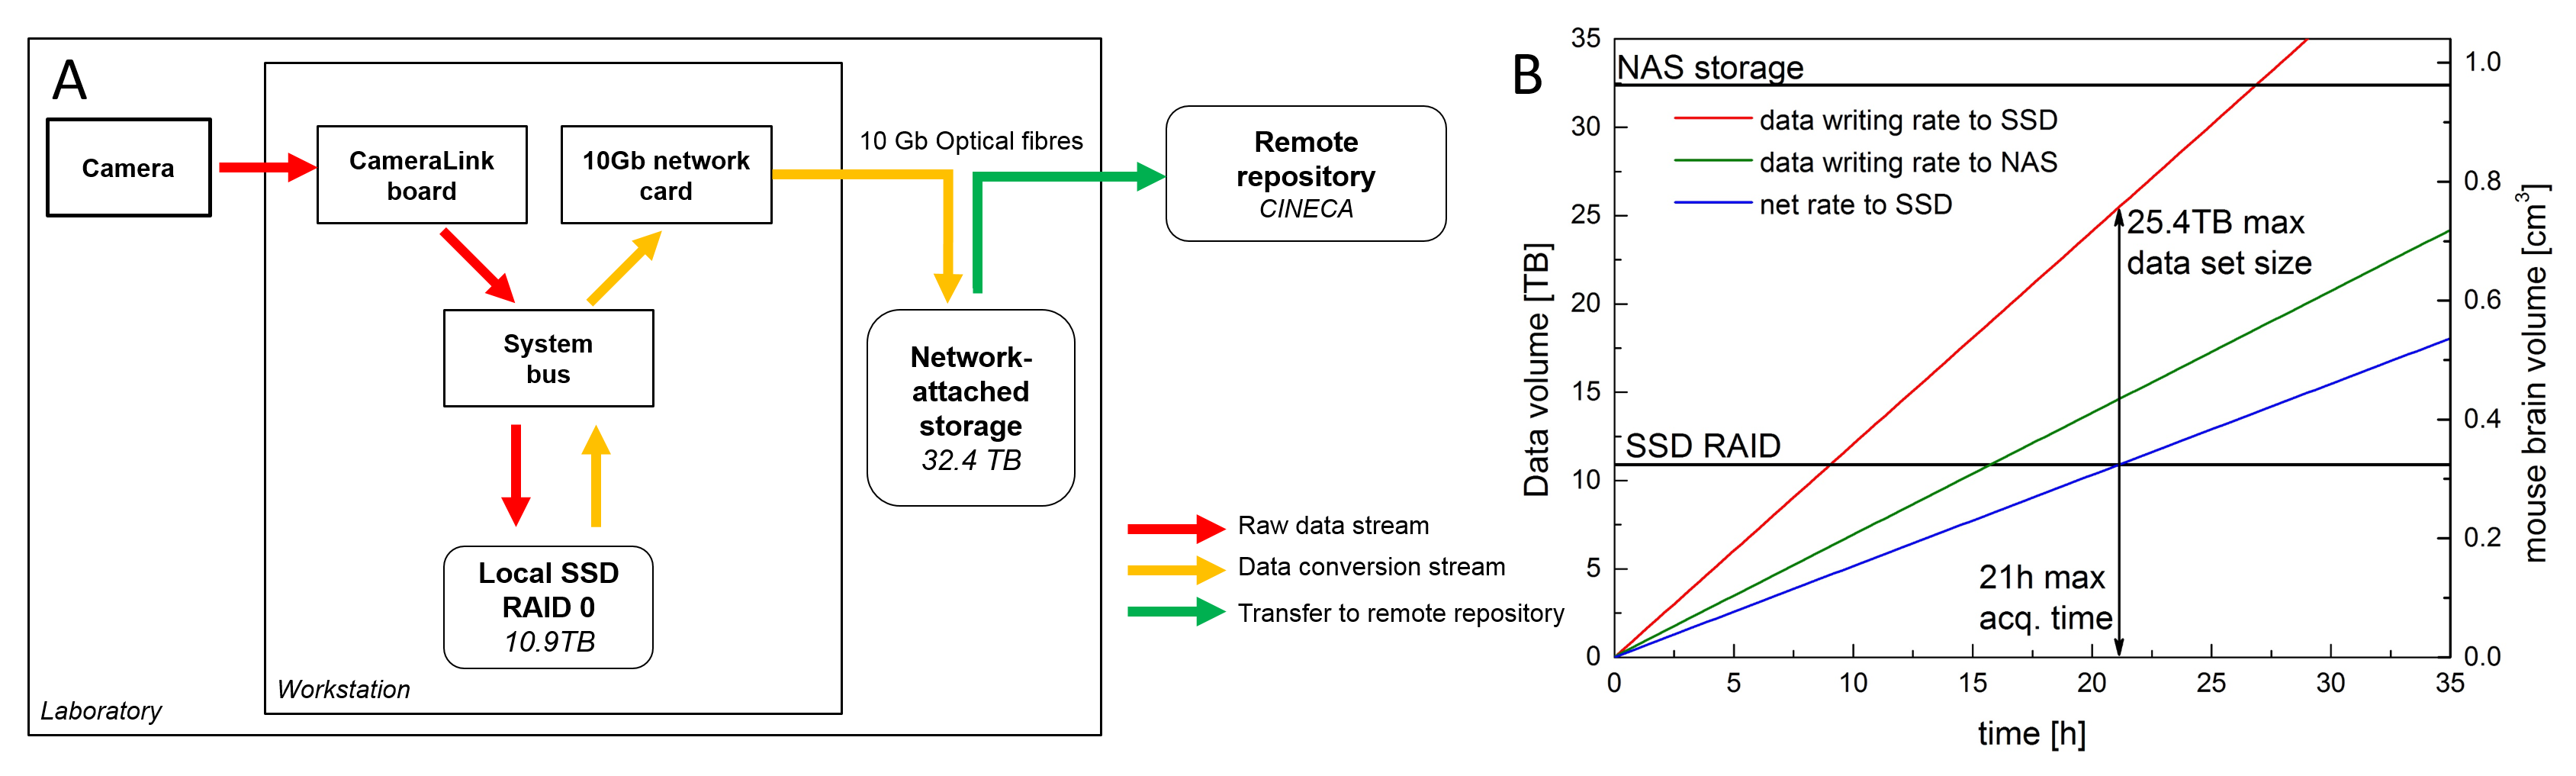
\includegraphics[width=\textwidth]{DataFlow.eps}
   \end{tabular}
   \end{center}
   \caption{\label{fig:DataFlow} Scheme of the data flow. (A) Data streaming on the microscope. The data is written through the CameraLink connection onto the SSD. From there the data can be transferred via a 10Gb connection to the NAS or to the supercomputing centre CINECA in Bologna. SSD: solid-state disk, RAID: redundant array of independent disks, NAS: network-attached storage. (B) Data production rate versus data conversion rate showing the maximum acquisition time and tomography size feasible before the SSD are filled up.} 
   \end{figure}
	
%\begin{landscape}
\begin{table}%[t!]
	\centering
		\caption[Data production]{Data production rates with two python scripts running in parallel.\label{tab:dataproduction}}
		\begin{tabular}{lrl}
		frame rate																	& 44			& Hz	\\
		size of 1 frame															& 8				& MB	\\
		frames per stack														& 3900		& 		\\
		size of original stack											& 30.4		& GB	\\
		size of converted stack											& 3				& GB	\\
		stack acquisition time											& 88.6		& s		\\
		stack conversion time												& 140			& s		\\
		time ratio conversion/ acquisition					& 1.6			& 		\\
		data production rate												& +1.2		&	TB/h\\
		data conversion rate												& -0.7		&	TB/h\\
		net rate																		& +0.5		&	TB/h\\
		SSD RAID																		& 10.9		& TB	\\
		max acquisition time to fill up SSDs				& 21			& h		\\
		max tomo size to fill up SSDs								& 25.4		& TB	\\
		\end{tabular}
\end{table}
%\end{landscape}
The unprecedented amount of data routinely produced by light sheet microscopy presents challenges to the traditional way we interact with our data. Having far passed the point of taking your data home with you on a hard drive at the end of the experiment, data management in light sheet microscopy requires a professional approach to centralised network architecture. The following paragraphs give an idea of the considerations one has to give to the big data volume problem. The camera used in our light sheet microscope has a dedicated work station with a CameraLink card and 10.9TB of SSD space in RAID 0 configuration. This finite storage capacity is further expanded by a network-attached storage (NAS) of 32.4TB (Figure\ref{fig:DataFlow}). The SSDs and the NAS are connected via a 10Gb bandwidth connection using a 10Gb switch and a 10Gb optical fibre connects our lab to the supercomputing centre CINECA in Bologna. Mention PICO system/storage analysis capacity there? Mention graphical processing unit and cores/processors/RAM of work station?
	
With the size of a single image of 8MB and a stack made up of say 3900 frames a single stack amounts to 30.4GB of disc space (see Table\ref{tab:dataproduction} for an overview of the values). Based on a frame rate of 44Hz each stack takes approximately 1.5 minutes to acquire and the SSD RAID fills up with a data writing rate of 1.2TB/h. If no further measures are taken the SSD RAID of 10.9TB would be filled up in just 9h. A custom compression script written in Python serves the triple purpose of translating the images from the proprietary Hamamatsu file format to 3D tif, to transfer the data from the SSD RAID to a network attached storage (NAS) and to reduce the raw data size by first, digitally downsampling the image resolution and second, applying a lossless compression to the tif images. This leads to a overall reduction of data size by a factor of ten, each stack now taking up only 3GB of disc space, albeit at a much slower conversion rate (-0.7TB/h) than the rate at which data is written to the SSD thus representing the most serious bottleneck to our data production pipeline. The SSD RAID fills up at a rate of 0.5TB/h which means the total acquisition time is limited to less than 24h and a total tomo size of just over 25TB. After this time acquisition has to be halted until the slower conversion process has caught up and freed the SSD RAID before data acquisition can start again. A whole mouse brain tomography would take 3 days of uninterrupted measuring yet with the necessary breaks for data transfer this time is easily doubled to tripled. 

	\subsection{Stitching and visualisation}
	
Given the limited field of view of the microscope, the acquisition of macroscopic specimens required many parallel image stacks to cover all the volume. Thus, in order to achieve a 3D image of the whole specimen from raw data, the Terastitcher\cite{Bria2012} has been recently proposed, i.e. a stitching tool capable to deal with teravoxel-sized images. However, the Terastitcher does not support input data acquired through the serial sectioning procedure, which leads to a specimen partitioned in different layers. Furthermore, only single channel images can be processed. For these reasons, we extended the Terastitcher functionalities introducing the two following additional features: i) stitching of a specimen partitioned in a number of overlapping layers for the hippocampus reconstruction and, ii) coping with images containing more than one channel for the human brain tomography.
With respect to the first requirement, that is allowing a complete reconstruction of a multi-layered raw data, we schematically depicts in Fig.1 the adopted strategy. First of all, the various input layers, each of which is composed of several parallel overlapping stacks, are separately stitched by using the existing Terastitcher tool. After this preliminary step,  leveraging the layer coordinates provided by the instrument, we import the processed layers as a new volume where each layer has a partial overlap with adjacent layers.  Furthermore, each layer is organized in a non-overlapping tiled format, enabling the application of a multi MIP-NCC approach\cite{Bria2012}, which computes the displacement  between two adjacent layers along all of the three directions (Fig. 1). When a displacement computation for each pair of adjacent layers has been computed, the overlapping regions are merged through a blending procedure which smooths the transition between layers, resembling once more the procedure used by Terastitcher for combining adjacent stacks. Finally, we note that due to the repositioning of each layer, the volume containing the reconstructed specimen might contain empty regions, which are thereby filled with black voxels. 
Turning our attention to the second additional feature, that is handling multi-channel images, the Terastitcher has been extended so that the MIP-NCC algorithm used for displacement computation can work on an image, which can be either 
the fusion of the input channels or one of the input channels. This permits to privilege the channel with more information content over the other channels as well as discard noisy channels. Note that the reconstructed 3D image can be produced with the same channel composition of raw data.


	\subsection{Example for postprocessing: Automated cell counting}
	See Reference\cite{Frasconi2014} for details.


\section{Data}

	\begin{figure}
   \begin{center}
   \begin{tabular}{c}
   \includegraphics[height=16cm]{LSMdata.eps}
   \end{tabular}
   \end{center}
   \caption{\label{fig:LSMdata} Whole mouse brain tomography. Imaging of whole transgenic mouse brains treated with CLARITY and cleared with TDE 63\% imaged with LSM (Olympus, 25X objective). (A) 3D rendering of a parvalbumin-dTomato brain. (B) 3D rendering of stacks from PV-dTomato mouse brain, GAD-dTomato mouse brain,  PI stained mouse brain, FITC-albumin labeled mouse brain, scale bar = 400 µm. (C,D,E,F) High resolution insert, of the stack corresponding to red boxes in C. Scale bar = 100 µm.} 
   \end{figure}
	
	Everybody take a look at Figure\ref{fig:LSMdata} because it is the best we have. 

\section{Conclusion}
summary
Light sheet microscopy has already been a game changer for large-scale imaging by yielding data with a combination of unprecedented spatio-temporal scale. The impact of this unique measurement technique will continue to revolutionise the field of whole brain connectomics due to its ability to record millions of images over the course of days or even weeks. The data produced in this fashion easily amounts several TB per data set and needs to be stored, transferred, retrieved, processed and visualised necessitating the concurrent development of novel computational interface and analysis methods. The latter need to be robust, standarised and fully automated processes yet allow for flexible, exploratory and tailored analysis. 

\section{Outlook}
where are we going next with this? ask Leo Onofri and Giulio to contribute to this, issues data mangament, aberration correction
mapping of complementary data sets obtained in the same system, eg structural connectivity, morphology and gene expression. 

\begin{landscape}
\begin{table}[t!]
	\centering
		\caption[Optomechanics]{Overview of optomechanical components.\label{tab:optomechanics}}
		\begin{tabular}{llll}
		Component												&	Manufacturer															& Part\# 								& Specifications 																													\\\hline
		\multirow{5}{*}[2.5em]{Lasers} 	& \multirow{5}{*}[2.5em]{Cobolt AB, Sweden} & MLD										& 405nm (for DAPI), 50mW, s-polarised																					 \\
																		&																						& MLD										& 445nm (for CFP), 50mW, s-polarised																					 \\
																		&																						& Calypso 							& 491nm (for GFP, FITC), 50mW, s-polarised																		 \\
																		&																						& Fandango							& 515nm (for Venus, YFP), 50mW, s-polarised																		 \\
																		&																						& Jive									& 561nm (for dTomato, PI, RFP), 50mW, s-polarised															 \\
		AOFT 														& AA Opto-Electronic, France								& AOTFnC-400.650-TN 		&	\pbox[t]{10.5cm}{$>90\%$ diffraction efficiency, 3nm resolution, low cross talk between laser lines, high separation angle}\\
		Laser modulator 								& Qioptiq	GmbH, Germany											& LM 0202 VIS ADP				& 400-650nm , $\nicefrac{\lambda}{2}$-voltage (633nm): 210V										 \\
		Pulse amplifier 								& Falco Systems, The Netherlands						& WMA-300								& 50x amplification up to $\pm$ 150V, DC to 5MHz signal bandwidth							 \\
		Galvo scanner 									& Cambridge Technology, USA									& 6220H 								& small angle step response $200\mu s$																				 \\		
		\multirow{2}{*}[0.6em]{Objectives}&	Nikon; Japan														& Plan Fluor EPI 				& 10x0.3NA, WD 17.5mm, EFL 20mm (excitation)																	 \\
																		& Olympus, Japan														& LMPLFLN20X 						& 20x0.4NA, WD 12mm, EFL 9mm (detection)																			 \\
		\multirow{3}{*}[0.6em]{Motor stages}& \multirow{2}{*}[0.6em]{Physik Instrumente, Germany}& C-863.11	& DC servo-motor controller																										 \\
																		&																						&	M-122									& Travel range 25mm, $0.1\micro m$ resolution, max. velocity 20mm/s						\\
																		&																						& M-116 								& Precision Rotation Stage, $2.5\micro rad$, max. velocity $20\degree /s$ 		\\
		Camera 													& Hamamatsu, Japan													& Orca Flash4.0 				& \pbox[t]{10.5cm}{sCMOS sensor, 2048(H) x 2048(V), cell dim.: $6.5\micro m$, active area: 13.3mm x 13.3mm, 16bit images}\\
		DAQ board												& National Instruments, USA									& NI PCIe-6353					& \pbox[t]{10.5cm}{AI: 1 MS/s multichannel; 16-bit resolution, ±10 V; AO: 2.86 MS/s, 16-bit resolution, ±10 V; digital I/O lines (hardware-timed up to 10 MHz), 100MHz max counter frequency}\\
		Workstation											& Dell, USA																	& T7500									&  \pbox[t]{10.5cm}{12GB RAM, Intel Xeon Processor X5647 @ 2.93 GHz, 64bit OS, Win7}\\
		\end{tabular}
\end{table}
\end{landscape}



		
\begin{landscape}
\begin{table}[t!]
	\centering
		\caption[Resolution]{Imaging properties and derived quantities. The thickness of the light sheet is approximately of the same size as the depth of field of the high NA detection lens.\label{tab:resolution}}
		\begin{tabular}{lrlrl}
		\multicolumn{5}{l}{Detection}\\\hline\hline
		wavelength																	&	$\lambda$				&																																					& 0.5			& $\mu m$	\\
		refractive index														&	n								&																																					& 1.45		& 				\\
		numerical aperture 													&	$\text{NA}_d$		&																																					& 1				& 				\\
		angular aperture 														& $\alpha$				&	$=sin^{-1}(\nicefrac{\text{NA}_d}{n})$																	& 43.6		& $deg$		\\
		magnification 															& M								&																																					& 25			&					\\
		tube lens 																	& $f_{\text{TL}}$	&																																					& 180			&	$mm$		\\
		effective focal length objective						& EFL							& $=\nicefrac{f_{\text{TL}}}{M}$																					& 7.2			& $mm$		\\
		diameter back focal plane										& BFP							& $= 2\text{EFL}\text{NA}_d$																							& 14.4		& $mm$		\\
		field number																& FN							&																																					& 18			& $mm$		\\
		field size in specimen											& S								& $=\nicefrac{\text{FN}}{M}$																							& 0.72		& $mm$		\\
		depth of field															& $\Delta$				& $=\nicefrac{\lambda*n}{(\text{NA}_d)^2}+ \nicefrac{n*e}{M \text{NA}_d}$	& 1.10 		& $\mu m$	\\ 
		Airy radius lat.														& $r_A$						& $=\nicefrac{0.61 \lambda}{\text{NA}_d}$																	& 0.31		& $\mu m$	\\\\
		\multicolumn{5}{l}{Excitation}\\\hline\hline
		numerical aperture 													&	$\text{NA}_e$		&																																					& 0.3			& 				\\
		magnification,	nominal											& m								&																																					& 10			&					\\
		tube lens 																	& $f_{\text{tl}}$	&																																					& 100			&	$mm$		\\
		effective focal length, objective						& efl							& $=\nicefrac{f_{\text{tl}}}{m}$																					& 20			& $mm$		\\
		magnification, effective										& $m_e$						&	$=\nicefrac{f_{\text{tl}}}{\text{efl}}$																	& 5				&					\\
		refractive index														&	$\eta$					&																																					& 1				& 				\\
		beam radius																	& $\omega$				&																																					& 4.5			& $mm$		\\
		%Airy radius lat.														& $r_a$						& $=\nicefrac{0.61 \lambda}{\text{NA}_e}$																	& 1.02		& $\mu m$	\\
		min light sheet waist												& $\omega_0$			& $=\nicefrac{\lambda \text{efl}}{\pi \omega}$														& 1.41		& $\mu m$	\\
		confocal parameter													& b								& $=\nicefrac{2 \pi \omega_0^2}{\lambda}$																	& 25.15		& $\mu m$	\\\\
		\multicolumn{5}{l}{Camera}\\\hline\hline
		cell size																		& e								&																																					& 6.5			&	$\mu m$	\\
		effective area 															& $r^2$						&																																					& $13.3^2$	&	$\text{mm}^2$	\\
		\end{tabular}
\end{table}
\end{landscape}		
		


		%\begin{landscape}
%\begin{table}[t!]
	%\centering
		%\caption[Optical clearing]{Overview of tools and chemicals necessary for optical clearing.\label{tab:clearing}}
		%\begin{tabular}{lllll}
		%Component												&	Manufacturer															& Part 						& Specs 					& Specs\\\hline
		%degasing chamber								& 																					&  	& 								& \\
		%clearing chamber								& 3D printed custom design									&  	& 								& \\
		%voltage supply									& 																					&  	& 								& \\
		%soap circulation thingy					& 																					&  	& 								& \\
		%shakey incubator								& 																					&  	& 								& \\
		%all those chemicals							& 																					&  	& 								& \\
		%\end{tabular}
%\end{table}
%\end{landscape}

%%------------- 
   %\begin{figure}
   %\begin{center}
   %\begin{tabular}{c}
   %\includegraphics[height=5.5cm]{fig2.eps}  % fig2 includes two images 
     %\\
     %(a) \hspace{5.1cm} (b)
   %\end{tabular}
   %\end{center}
   %\caption 
   %{ \label{fig:example2} %>> use \label inside caption to get Fig. number with \ref{}
%Example of a figure containing multiple images: (a) sun and (b) blob. Figures containing multiple images must be submitted to SPIE as a single image file.} 
   %\end{figure} 

%%%%%%%%%%%%%%%%%%%%%%%%%%%%%%%%%%%%%%%%%%%%%%%%%%%%%%%%%%%%%
\acknowledgments 
Human Brain Project tutta la vita. 
GARR gave us a beautiful 10gb fiber to cineca
CINECA for hosting us on pico

%%%%%%%%%%%%%%%%%%%%%%%%%%%%%%%%%%%%%%%%%%%%%%%%%%%%%%%%%%%%%
%%%%% References %%%%%

%\bibliography{report2}   %>>>> bibliography data in report.bib
\bibliographystyle{spiejour}   %>>>> makes bibtex use spiejour.bst
\begin{thebibliography}{0}

\bibitem{Huisken2009} J. Huisken and D. Y. Stainier, ``Selective plane illumination microscopy techniques in developmental biology," \emph{Development} \textbf{136}(), 1963–1975 (2009).

\bibitem{Chung2013} Chung, K., Wallace, J., Kim, S. Y., Kalyanasundaram, S., Andalman, A. S., Davidson, T. J. \& Deisseroth, K. Structural and molecular interrogation of intact biological systems. \emph{Nature} \textbf{497}, 332–33 (2013).

\bibitem{Tomer2014} Tomer, R., Ye, L., Hsueh, B. \& Deisseroth, K. Advanced CLARITY for rapid and high-resolution imaging of intact tissues. \emph{nature protocols} \textbf{9}, 1682-1697 (2014).

\bibitem{Silvestri2012} L. Silvestri, A. Bria, L. Sacconi, G. Iannello,  and F. S. Pavone,  ``" \emph{Opt Express} \textbf{20}(), 20582-20598 (2012).

\bibitem{Frasconi2014} P. Frasconi, L. Silvestri, P. Soda, R. L. Cortini, F. S. Pavone and G. Iannello, ``" \emph{Bioinformatics} \textbf{30}(), i587-i593 (2014).

\bibitem{Bria2012} A. Bria and G. Iannello,  ``TeraStitcher-A tool for fast automatic 3D-stitching of teravoxel-sized microscopy images,"  \emph{BMC bioinformatics} \textbf{13}(), 316 (2012).

\end{thebibliography}


\listoffigures
%pannel1: optical pathway, drawing images from chamber, sample mirror photos
%pannel2: software scheme
%panel3: hardware connection scheme
%panel4: data pipeline, graph data amount/time
%panel5: experiment pipeline
%panel6: images, tomos



\listoftables

%\end{spacing}
\end{document} 
